\section{Damping, settling time and shock tolerance}

\subsection*{Q4 -- Settling time with combined damping}

Independent loss channels add in parallel: damping coefficients sum, quality
factors combine as reciprocals.

\paragraph{Air damping.} The top-side area of the moving structure
\textcolor{blue}{(the same two plates, column and $20$ fingers used for the
mass)} is
\begin{equation}
  A_{m}=\textcolor{blue}{2}L W_{m} + L_{m} W_{m} + \textcolor{blue}{20}\, L_{c} W_{c}
      = \textcolor{blue}{\SI{7.60e-9}{\meter\squared}},
\end{equation}
giving an air damping coefficient
\begin{equation}
  b_{\mathrm{air}}=c_{\mathrm{air}}\,A_{m}=\textcolor{blue}{\SI{1.23e-7}{\newton\second\per\meter}},
  \qquad
  Q_{\mathrm{air}}=\frac{\sqrt{km}}{b_{\mathrm{air}}}=\textcolor{blue}{97}.
\end{equation}

\paragraph{Clamping loss.} From the given $Q_{\mathrm{clamping}}=500$,
\begin{equation}
  b_{\mathrm{clamp}}=\frac{\sqrt{km}}{Q_{\mathrm{clamping}}}
                   =\textcolor{blue}{\SI{2.39e-8}{\newton\second\per\meter}}.
\end{equation}

\paragraph{Combined damping.}
\begin{equation}
  b=b_{\mathrm{air}}+b_{\mathrm{clamp}}=\textcolor{blue}{\SI{1.47e-7}{\newton\second\per\meter}},
  \qquad
  \frac{1}{Q}=\frac{1}{Q_{\mathrm{air}}}+\frac{1}{Q_{\mathrm{clamping}}}
  \;\Rightarrow\; Q\approx \textcolor{blue}{81.5}.
\end{equation}
Air damping dominates (\textcolor{blue}{$Q_{\mathrm{air}}\!=\!97 \ll Q_{\mathrm{clamping}}\!=\!500$}),
so $Q$ is essentially set by the surrounding gas.
\textcolor{blue}{The corrected $Q\approx81.5$ is, reassuringly, close to the
$Q=83$ that Part~2 imposes on the FEM model.}

\paragraph{Settling time.} With \textcolor{blue}{$\zeta = b/(2\sqrt{km})=1/(2Q)\approx 6.1\times10^{-3}$}
the system is strongly underdamped. Its envelope decays as $e^{-\zeta\omega_{0}t}$,
giving a $\pm 5\%$ settling time of
\begin{equation}
  t_{s} \;\approx\; \frac{-\ln(0.05)}{\zeta\,\omega_{0}}
              \;=\; \frac{3.00}{\zeta\,\omega_{0}}
              \;\approx\; \textcolor{blue}{\SI{145}{\micro\second}}.
\end{equation}
Figure~\ref{fig:step} shows the simulated response for a 1\,nN step input.

\begin{figure}[H]
\centering
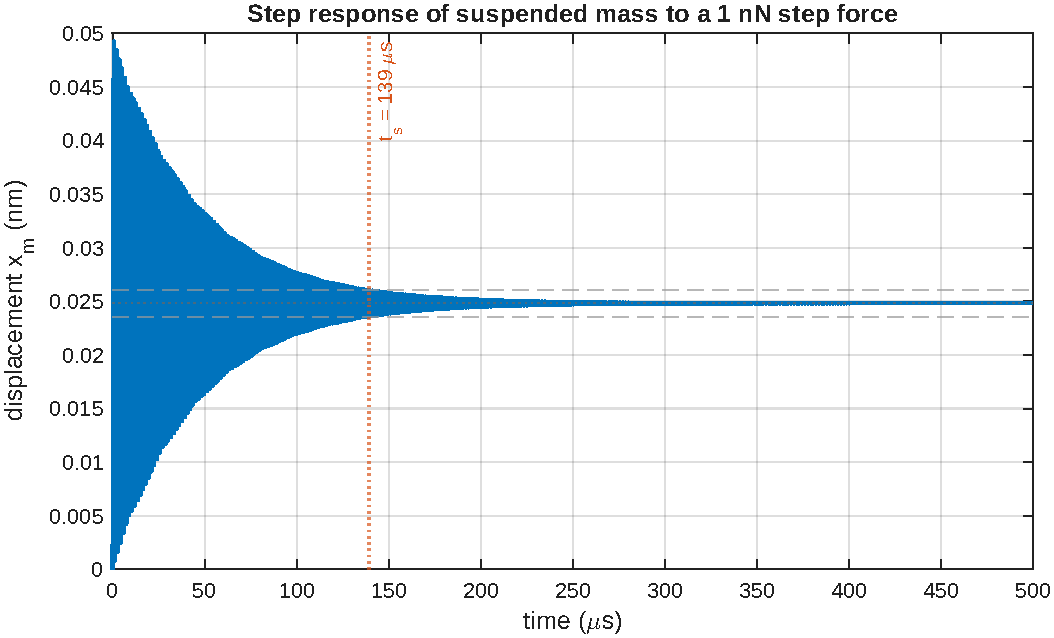
\includegraphics[width=0.78\textwidth]{figures/q4_step_response.pdf}
\caption{Step response to a 1\,nN input force. The dashed lines mark the
$\pm 5\%$ band around the steady-state value $F_{0}/k$. Settling occurs after
roughly $t_{s}\approx \textcolor{blue}{\SI{145}{\micro\second}}$.}
\label{fig:step}
\end{figure}

\subsection*{Q5 -- Maximum tolerable harmonic acceleration}

A harmonic base acceleration $a(t)=A\cos(\omega t)$ acts on the suspended mass
as an inertial force $-m a$. With $\Vd=0$ (no electrostatic force), the
equation of motion in the frequency domain is
\begin{equation}
  (k - m\omega^{2} + j\omega b)\,X(j\omega) = -m\,A(j\omega),
\end{equation}
so the magnitude of the displacement is
\begin{equation}
  |X(j\omega)| \;=\; \frac{m\,|A(j\omega)|}
                          {\sqrt{(k-m\omega^{2})^{2}+(\omega b)^{2}}}.
\end{equation}
The mass touches the waveguide when $|X|=g_{0}$. The maximum tolerable
acceleration as a function of frequency is therefore
\begin{equation}
  \boxed{\;
    A_{\max}(\omega) \;=\; \frac{g_{0}}{m}
      \sqrt{(k-m\omega^{2})^{2}+(\omega b)^{2}}.
  \;}
  \label{eq:Amax}
\end{equation}

\paragraph{DC limit ($\omega\to 0$).}
\begin{equation}
  A_{\max,\mathrm{DC}} \;=\; \frac{g_{0} k}{m} \;=\; g_{0}\,\omega_{0}^{2}
   \;\approx\; \textcolor{blue}{\SI{2.28e6}{\meter\per\second\squared}}
   \;\approx\; \textcolor{blue}{\SI{2.3e5}{\textit{g}}}.
\end{equation}

\paragraph{Worst-case AC frequency ($\omega = \omega_{0}$).} At resonance the
square root reduces to $\omega_{0} b$, so
\begin{equation}
  A_{\max,\mathrm{res}} \;=\; \frac{g_{0}\,\omega_{0}\,b}{m}
                          \;=\; \frac{g_{0}\,\omega_{0}^{2}}{Q}
                          \;\approx\; \textcolor{blue}{\SI{2.79e4}{\meter\per\second\squared}}
                          \;\approx\; \textcolor{blue}{\SI{2.8e3}{\textit{g}}}.
\end{equation}
Resonance reduces shock tolerance by a factor $Q$. The DC value
($\sim\!10^{5}\,g$) is enormous, but at $f_{0}$ the device is roughly
\textcolor{blue}{$80\times$} more vulnerable. Fig.~\ref{fig:amax} plots $A_{\max}(f)$.

\begin{figure}[H]
\centering
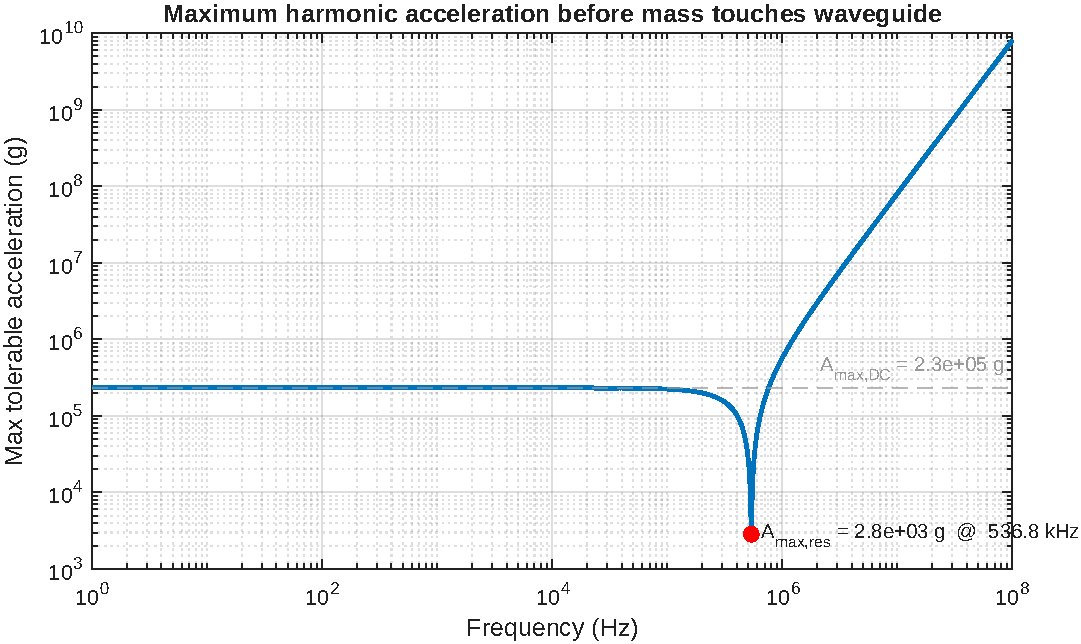
\includegraphics[width=0.78\textwidth]{figures/q5_amax.pdf}
\caption{Maximum tolerable acceleration before the suspended mass contacts
the waveguide, computed from Eq.~\ref{eq:Amax}. The minimum lies at
$f_{0}\approx \textcolor{blue}{\SI{537}{\kilo\hertz}}$, where the device is most sensitive to
mechanical excitation.}
\label{fig:amax}
\end{figure}
